\documentclass[problem]{mcs}

\begin{pcomments}
  \pcomment{PS_3color_crossover_SAT}
  \pcomment{by ARM 4/6/14}
\end{pcomments}

\pkeywords{
  coloring
  planar
  3-coloring
}

%%%%%%%%%%%%%%%%%%%%%%%%%%%%%%%%%%%%%%%%%%%%%%%%%%%%%%%%%%%%%%%%%%%%%
% Problem starts here
%%%%%%%%%%%%%%%%%%%%%%%%%%%%%%%%%%%%%%%%%%%%%%%%%%%%%%%%%%%%%%%%%%%%%

\begin{problem}
The 3-coloring problem for planar graphs turns out to be no easier
than the 3-coloring problem for arbitrary graphs.  This claim follows
very simply from the existence of a ``3-color cross-over gadget.''
Such a gadget is a planar graph whose outer face is a cycle with four
designated vertices $u,v,w,x$ occurring in clockwise order such that

\begin{enumerate}

\item\label{exist3coloring} Any assignment of colors to vertices $u$ and $v$ can be
  completed into a 3-coloring of the gadget.
\item\label{colors-cross} In every 3-coloring of the gadget, the colors of $u$ and $w$ are
  the same, and the colors of $v$ and $x$ are the also same.

\end{enumerate}

Figure~\ref{fig:3color-gadget} shows such a 3-color cross-over
gadget.\footnote{This gadget and reduction of 3-colorability to planar
  3-colorability are due to Larry Stockmeyer~\cite{Stockmeyer73}.}

\begin{figure}\inbook{[h]}
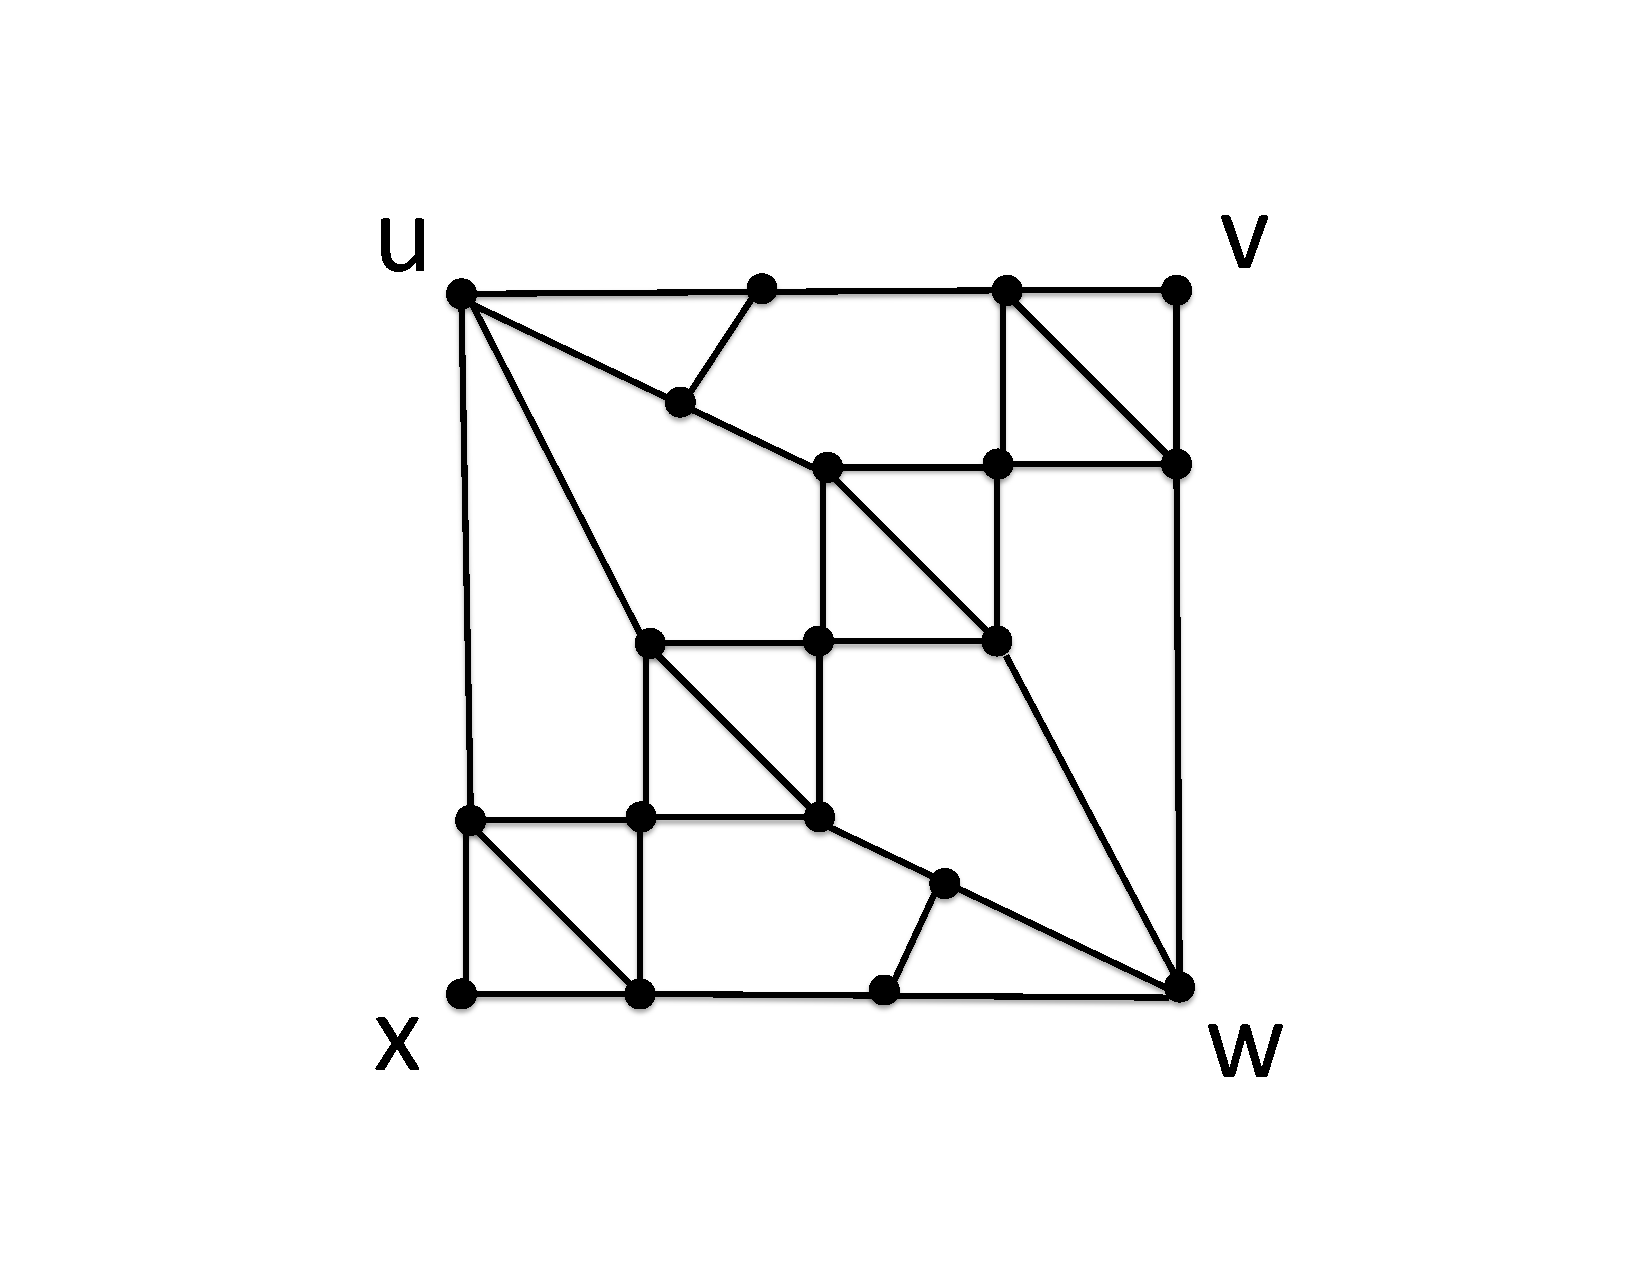
\includegraphics[width=3.5in]{3color-crossover-gadget}
\caption{A 3-color cross-over gadget.}
\label{fig:3color-gadget}
\end{figure}

So to find a 3-coloring for \emph{any} simple graph, simply draw it in
the plane with edges crossing as needed, and then replace each
occurrence of an edge crossing by a copy of the gadget as shown in
Figure~\ref{fig:replace-crossing}.  This yields a planar graph which
has a 3-coloring iff the original graph had one.

\begin{figure}\inbook{[h]}
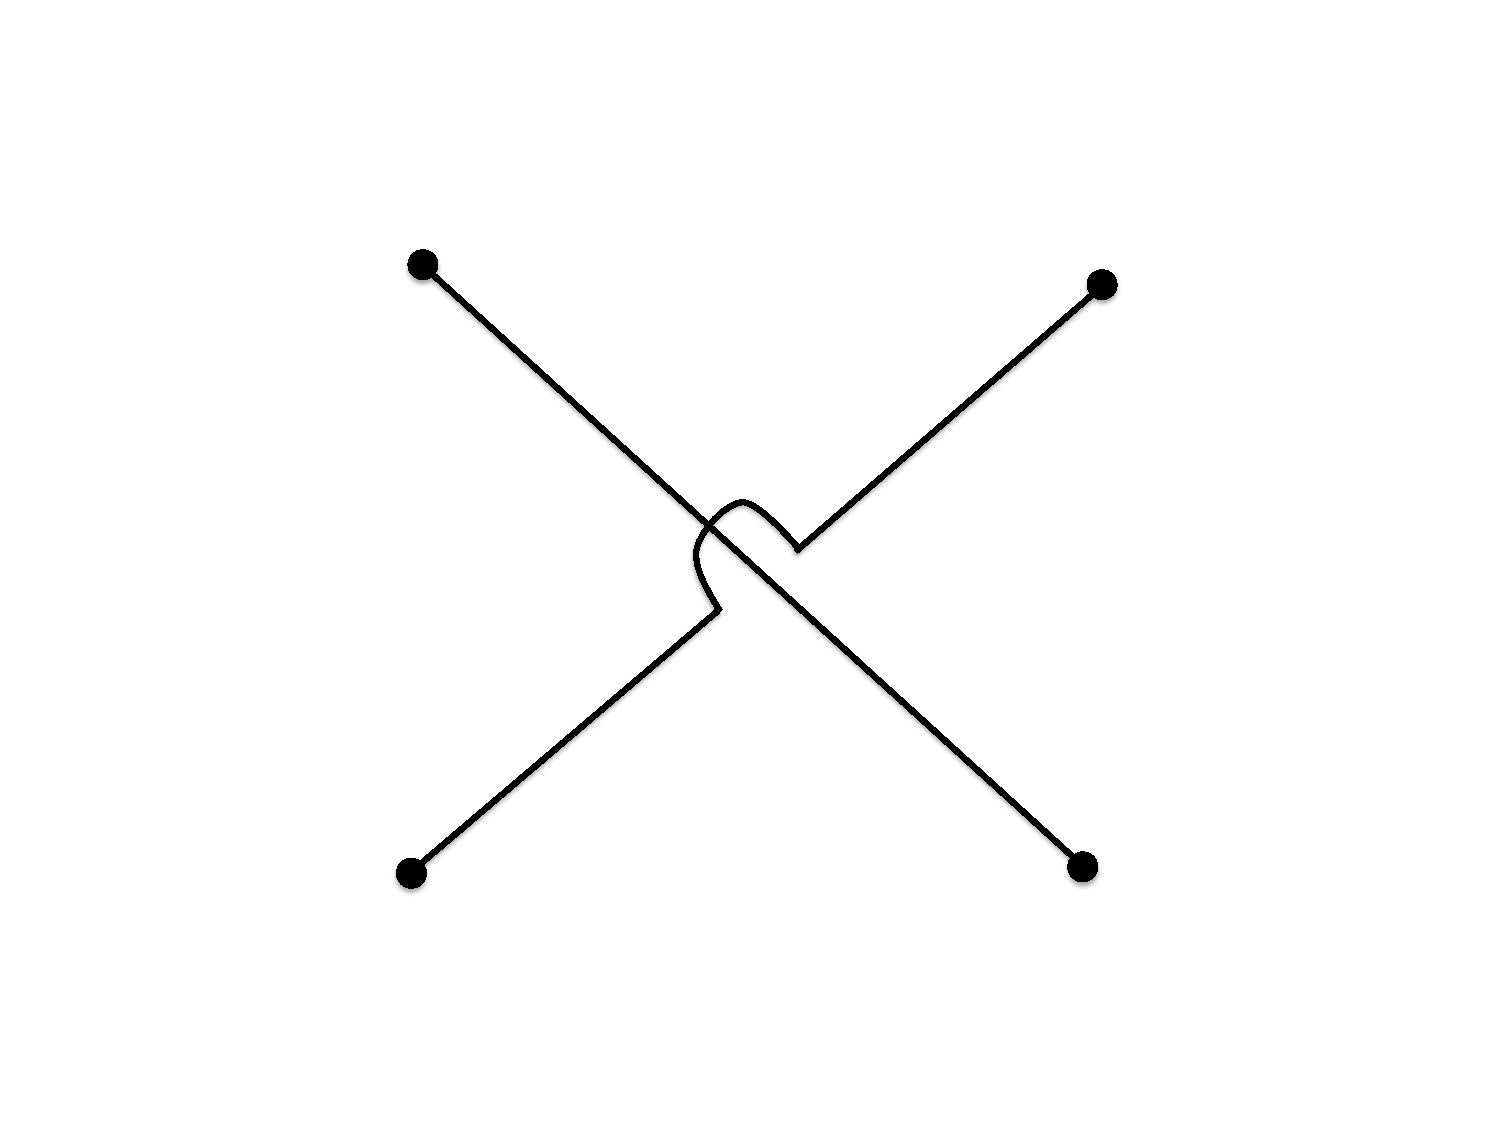
\includegraphics[width=2.3in]{edge-crossing} 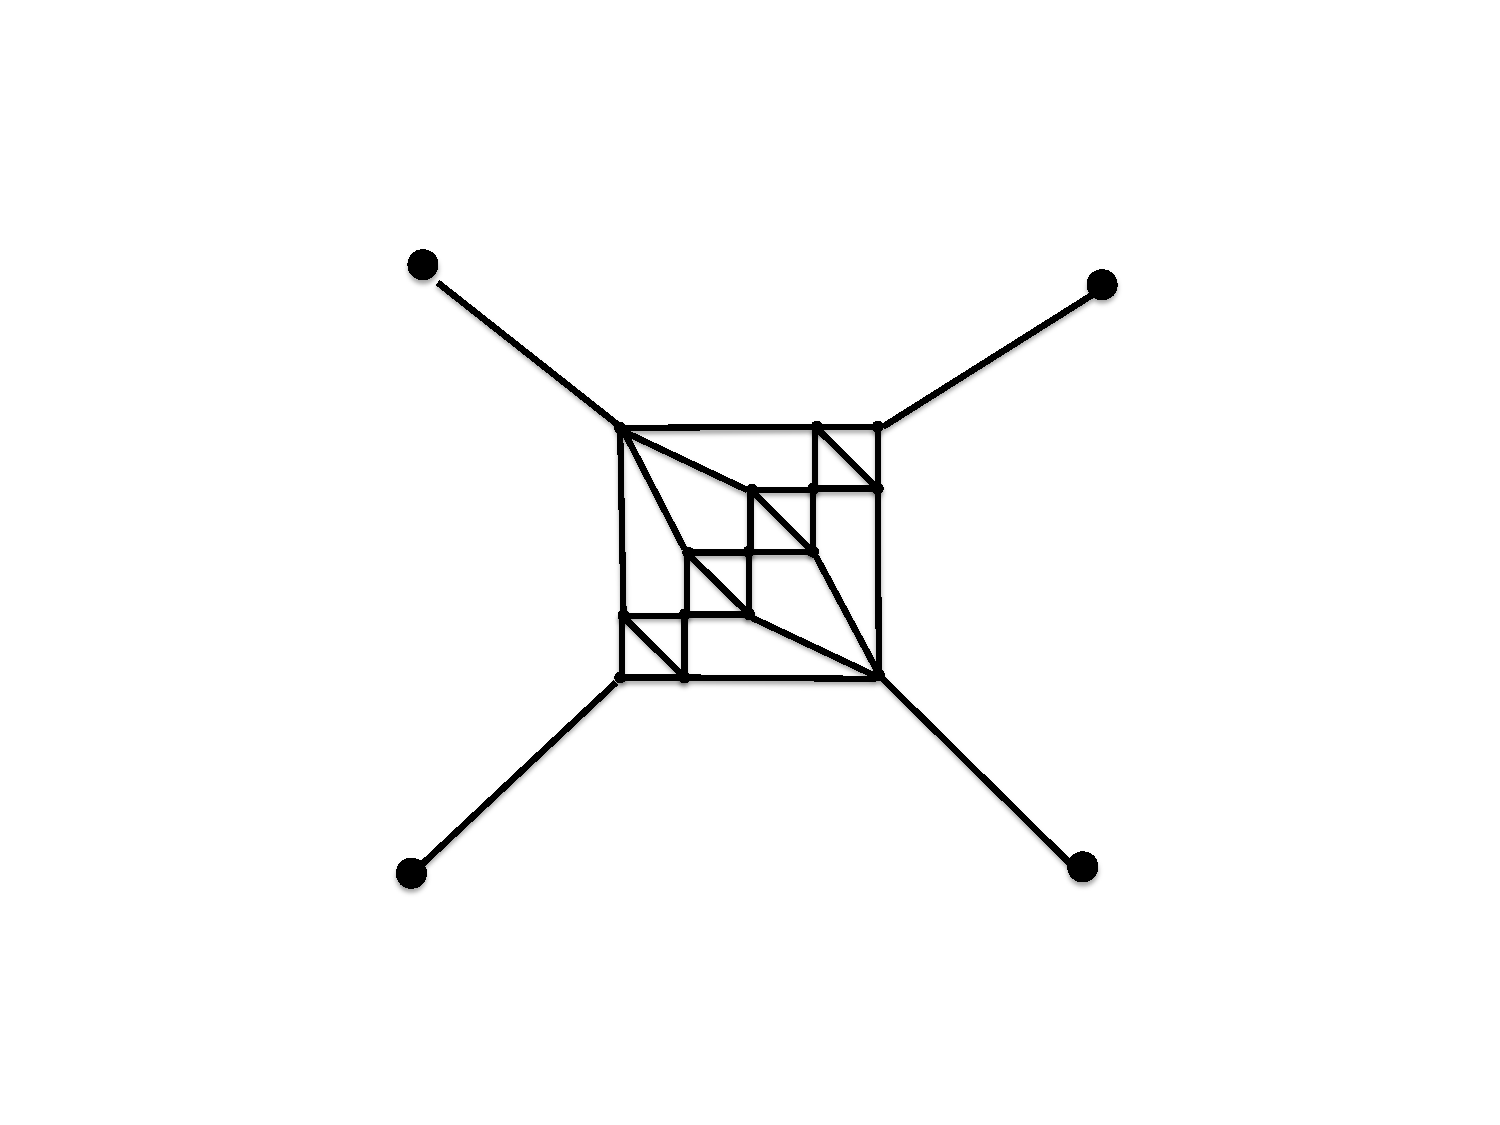
\includegraphics[width=2.3in]{3color-gadget-crossing}
\caption{Replacing an edge-crossing with a planar gadget.}
\label{fig:replace-crossing}
\end{figure}

\bparts

\ppart\label{verify3coloring} Prove that the graph in
Figure~\ref{fig:3color-gadget} satisfies
condition~\eqref{exist3coloring} by exhibiting the claimed
3-colorings.

\hint Only two colorings are needed, one where $u$ and $v$ are the
same color and another where they are not the same color.

\begin{solution}
\begin{figure}\inbook{[h]}
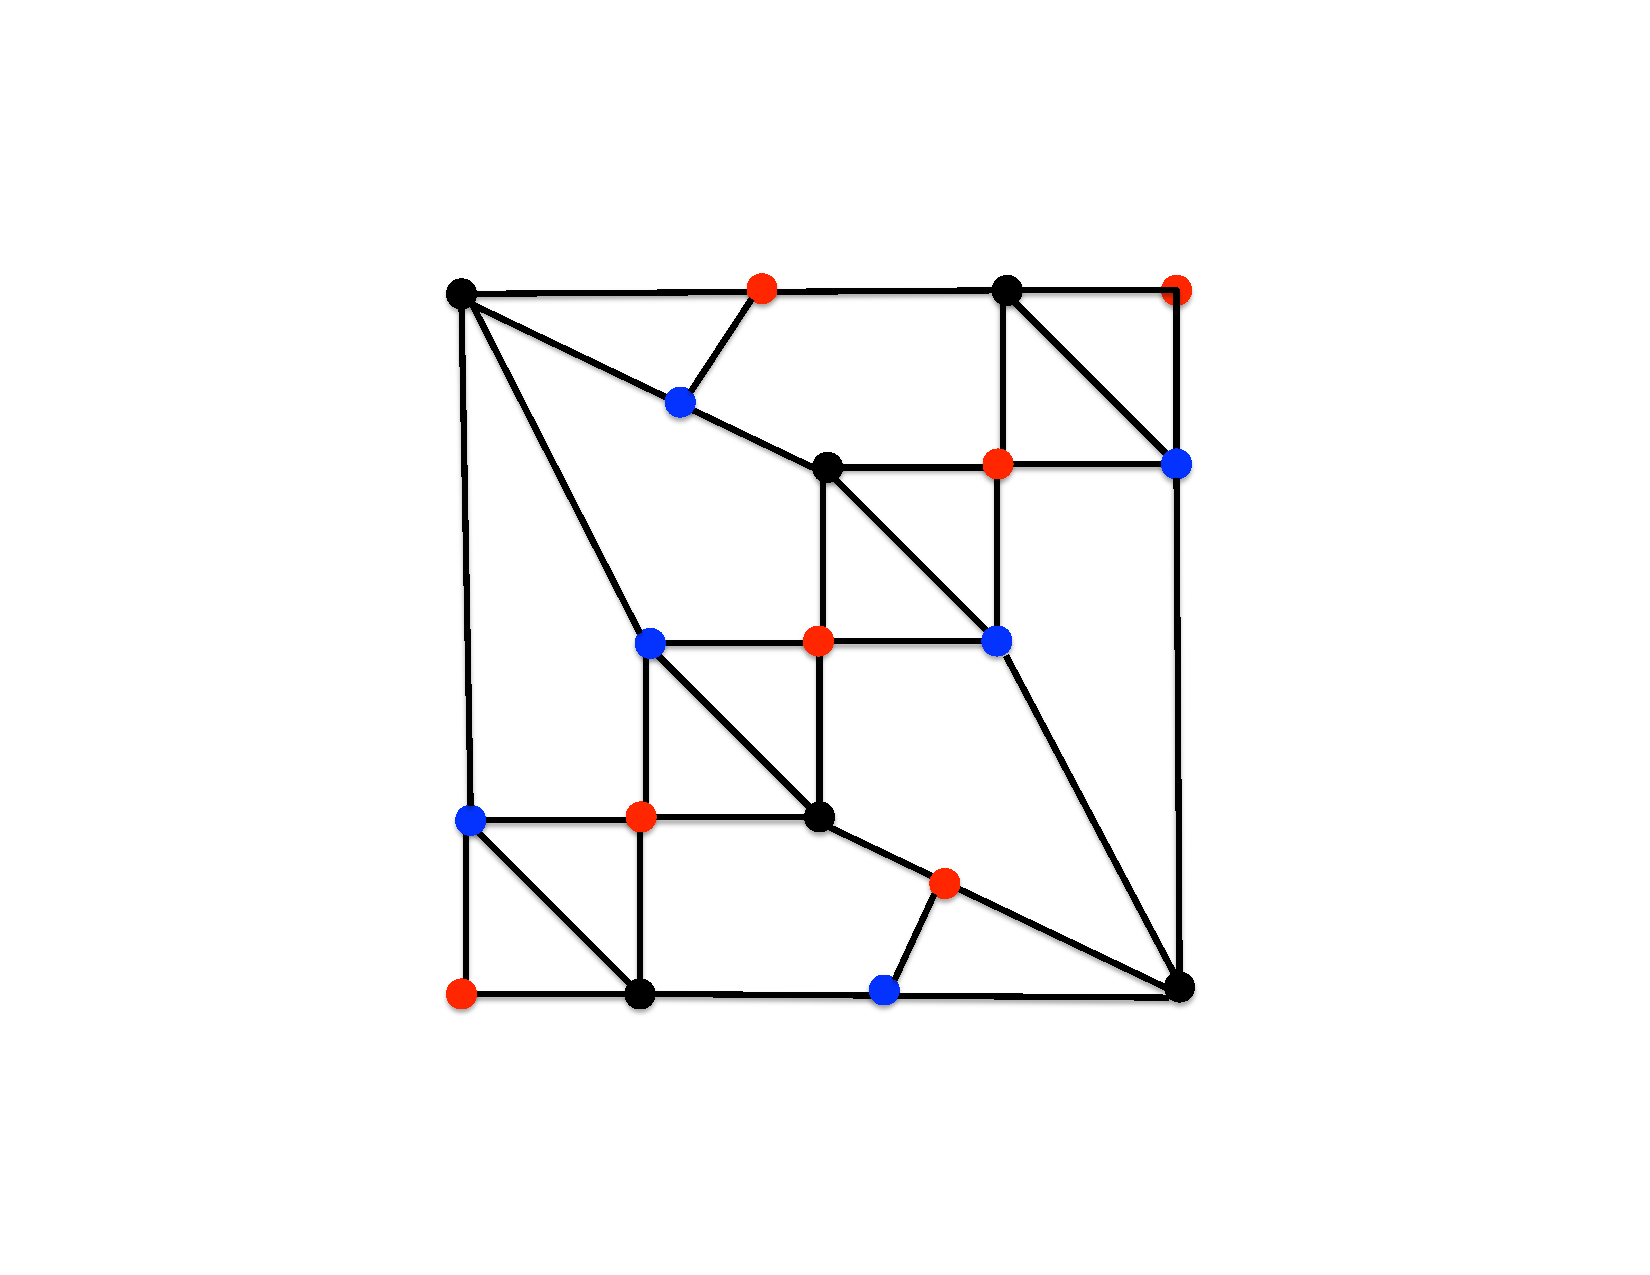
\includegraphics[width=2.3in]{3color-diffcolor-cross} 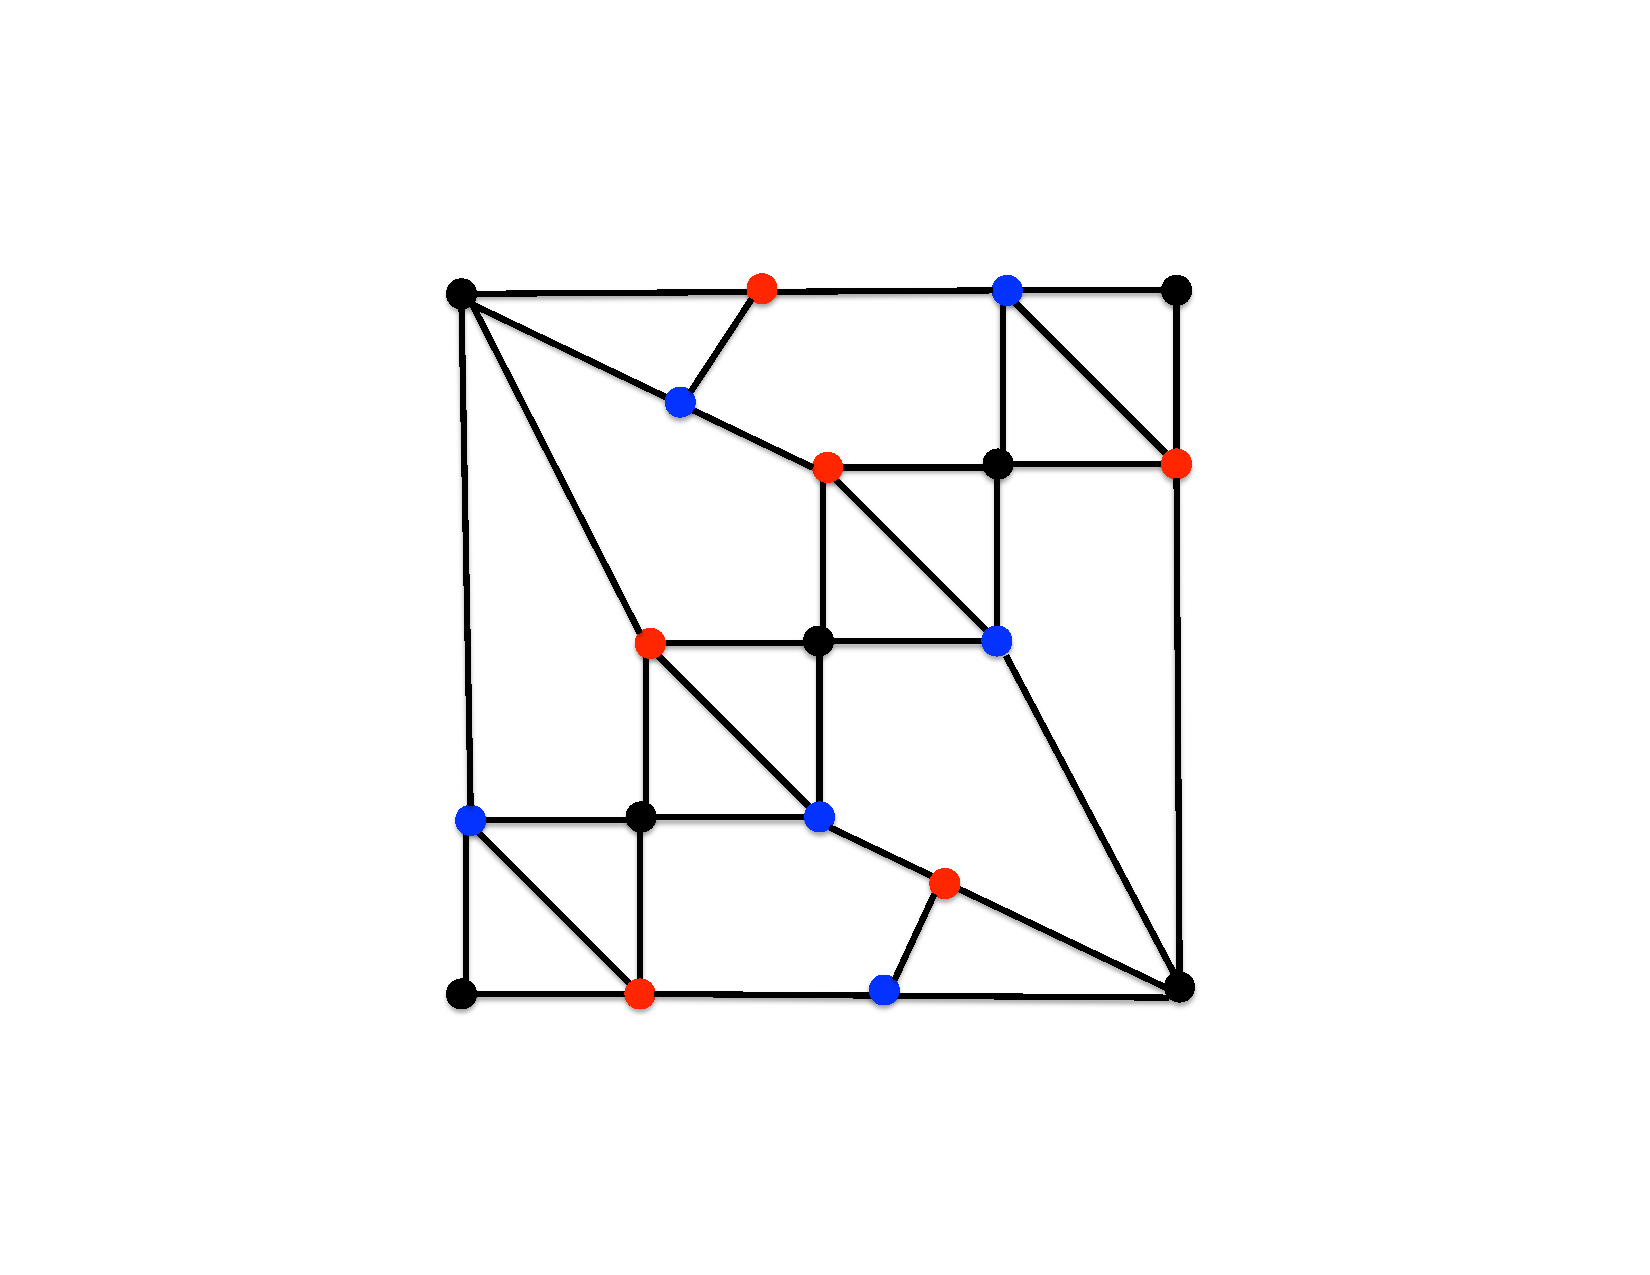
\includegraphics[width=2.3in]{3color-samecolor-cross}
\caption{3-colorings for the gadget.}
\label{fig:3colorings}
\end{figure}
\end{solution}

\ppart Prove that the graph in Figure~\ref{fig:3color-gadget}
satisfies condition~\eqref{colors-cross}.

\hint The colorings for part~\eqref{verify3coloring} are almost
completely forced by the coloring of $u$ and $v$.

\begin{solution}
\TBA{TBA}
\end{solution}

\eparts

\end{problem}

%%%%%%%%%%%%%%%%%%%%%%%%%%%%%%%%%%%%%%%%%%%%%%%%%%%%%%%%%%%%%%%%%%%%%
% Problem ends here
%%%%%%%%%%%%%%%%%%%%%%%%%%%%%%%%%%%%%%%%%%%%%%%%%%%%%%%%%%%%%%%%%%%%%

\endinput
